\chapter{Umsetzung in RoboCup2D}
    % ``Was ist RoboCup'' \\
    % ``Was für Ligen gibt es'' \\
    % ``Was für eine Domäne ist es im Vergleich zu anderen'' \\
    % \\
    RoboCup ist ein Fußball Simulator, der seine Anfänge in 1993 in Japan, Tokyo gefunden hat. Eine Gruppe von Forschern, inklusive Minoru Asada, Yasuo Kuniyoshi und Hiroaki Kitano, haben als einen Wettbewerb unter dem Namen \textbf{Robot J-League} gestartet. Der Name stammt von einer professionellen japanischen Fußball Liga.\\
    \\
    Nach einem Monat haben sie jedoch weltweit überwältigendes Feedback bekommen und haben die Initiative als internationales Projekt weitergeführt, daher kam die Umbenennung zur \textbf{Robot World Cup Initiative}, kurz RoboCup. \\
    % \textit {(source: http://www.robocup.org/about-robocup/a-brief-history-of-robocup/)} \\
    \\
    Die RoboCup Initiative hat betreibt derzeit sechs große Wettbewerbe, die sich jeweils wieder in Ligen und Subligen aufteilen lassen. Darunter fällt \textbf{RoboCup Soccer}, \textbf{RoboCup Rescue Rescue}, \textbf{RoboCup Junior}, \textbf{RoboCup Logistics}, \textbf{RoboCup @ Work} und \textbf{RoboCup @ Home}. Unsere Implementierung fällt in die Subliga \textbf{2D Soccer Simulation}, in der es darum geht in einer zweidimensionalen Welt zwei Fußballmannschaften gegeneinander antreten zu lassen.\\
    \\
    Die Aufgabe die wir angehen gehört zu einem Fragement von RoboCup2D, genannt \textbf{Half Field Offense}.\\

    \begin{figure}[htbp]
        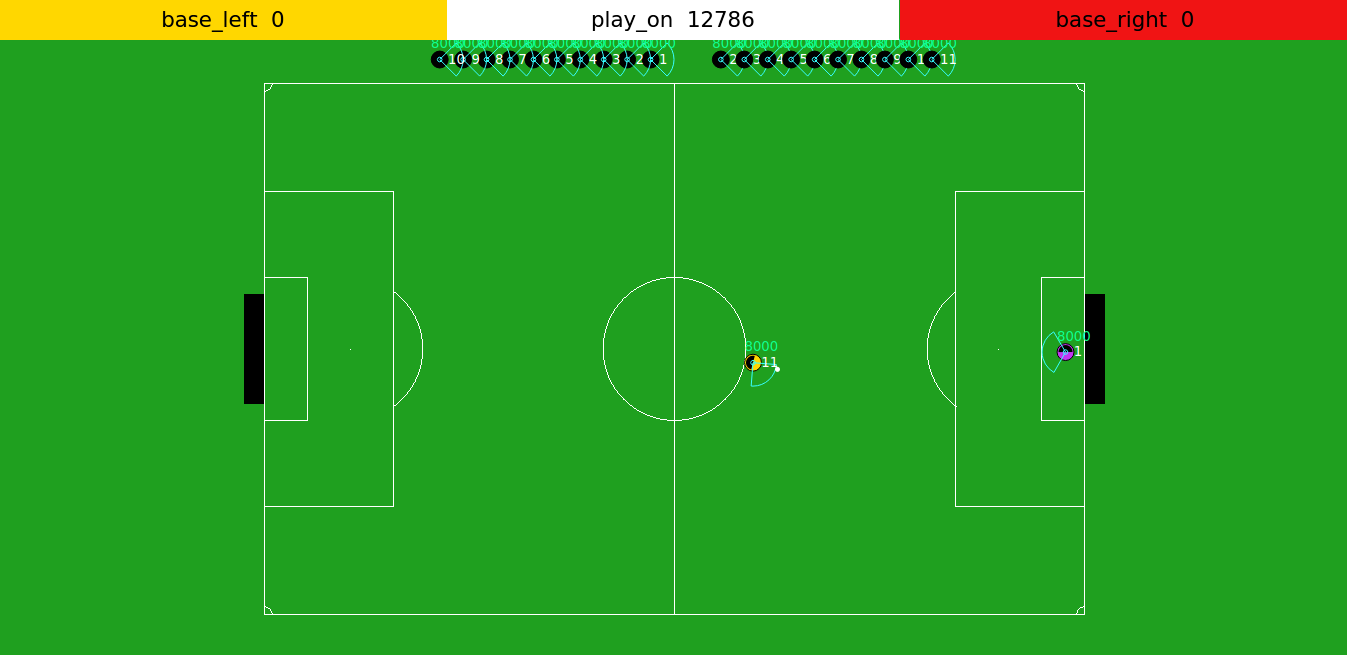
\includegraphics[width = 1.0\textwidth, center]{../pictures/full-field.png}
        \caption{Screenshot von dem gesamten Spielfeld von RoboCup2D \label{fig:somelabel}}
    \end{figure}

    \section{Half Field Offense}
        % ``Was ist Half Field Offense'' \\
        % ``Wie ist das Spielfeld aufgebaut'' \\
        % ``Warum wurde diese Domäne gewählt'' \\

        Die Domäne Half Field Offense grenzt das Spielfeld auf eine Hälfte ein, sodass wir 4 Angreifer und 3 Verteidiger + Torwart haben. Diese Einschränkung vereinfacht den Such- und Zustandsraum immens und erlaubt potenziell eine Wiederverwendbarkeit der Agenten, wenn eine vollständige Mannschaft aufgebaut wird.\\
        \\
        In unserer Implementierung haben wir lediglich ein 1v1 Szenario, also ein Angreifer gegen ein Torwart. Diese sieht jedoch explizit ein nahtlosen Skalierung auf ein 4vs4 Szenario vor, sodass weitere Parametrisierung ohne viel Aufwand ausprobiert werden können.\\

        \begin{figure}[htbp]
            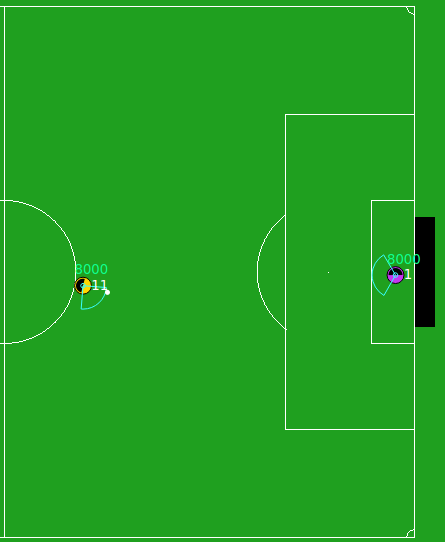
\includegraphics[width = 0.5\textwidth,height = 0.4\textheight, center]{../pictures/half-field.png}
            \caption{Screenshot von dem Spielfeld für den Subtask HFO \label{fig:somelabel}}
        \end{figure}
        \noindent
        Im Folgenden wir die Domäne samt Zustandsraum und Aktionen erklärt, sowie ihren Einschränkungen für die Anwendung von Machine Learning Algorithmen.\\
        % \cite{ http://www.cs.utexas.edu/users/ai-lab/?hausknecht:aamasws16 }
\newpage
        \subsection{Zustandsraum}
            % ``Unterschiedliche Zustandsräume, kommt drauf an wie viele Spieler aufm Feld sind (zitat vom HFO Paper)''\\
            % ``Angepasst für Maschinen (zitat HFO)'' \\
            % ``Umrechnung für Menschen'' \\
            % ``Fullstate flag''
            Der Zustandsraum der HFO Domäne kann in den \textbf{High Level State} und den \textbf{Low Level State} aufgeteilt werden. Der Unterschied ist lediglich in der Dimensionalität, da man aus dem Low Level State den High Level State ableiten kann. Die Zustandsräume werden durch folgende Formeln aufgespannt:\\
            \\
            \textit{Sei T die Anzahl der Teammitglieder, O die Anzahl der Gegner:}
            \begin{center}
                \textit{High Level State} $ := 10 + 6T + 3O \hspace{10mm} $ \\
                \textit{Low Level State}  $ := 58 + 8T + 8O \hspace{9mm} $ \\
            \end{center}
%            \textit{(Frage: Alles vom Paper abschreiben oder referenzieren?)} \\
 %           \\
            In unserem 1v1 High Level Setting haben wir damit 13 Zustandsparameter. Vier von diesen Parametern gehören zu dem Torwart, aber da seine Position implizit durch andere Ausprägungen gegeben ist, werden sie nicht beachtet. Redundante Information würde den Suchraum unnötig aufblähen und die Suche verlängern. Folgende 9 Zustände wurden bereitgestellt:

            \begin{table}[H]
                \begin{center}
                \hspace*{-1.5cm}
                \begin{tabular}{ |l|c|c|c| } 
                    \hline
                    \hfill Zustandsbeschreibung & Wertebereich & Kontinuierlich & Bool'sch \\ \hline
                    x Koordinaten & $[ -1, +1 ]$ & X & \hfill \\ \hline
                    y Koordinaten & $[ -1, +1 ]$ & X & \hfill \\ \hline
                    Sichtrichtung & $[ -1, +1]$ & X & \hfill \\ \hline
                    Nähe zum Ball & $[ -1, +1 ]$ & X & \hfill \\ \hline
                    Winkel zum Ball & $[ -1, +1 ]$ & X & \hfill \\ \hline
                    Kann eine Ballaktion ausgeführt werden & $[ -1, +1 ]$ & \hfill & X \\ \hline
                    Winkel zum Mittelpunkt des Tors & $[ -1, +1 ]$ & X & \hfill \\ \hline
                    Größte offene Winkel zwischen Torwart und Torpfosten & $[ -1, +1 ]$ & X & \hfill \\ \hline
                \end{tabular}
                \end{center}
                \caption{Zustandsraum von HFO 1vs1 \label{fig:somelabel}}
            \end{table}

            \hspace*{-1.5cm}
            \textit{(Muss hier eine Erklärung wie der Zustand kodiert war hin, also Normalisierung der Winkel?\\
            \hspace*{-1.5cm} Wäre dann eigentlich abschreiben ab 15.1.1 von https://github.com/LARG/HFO/blob/master/doc/manual.pdf)}
            % (src: https://github.com/LARG/HFO/blob/master/doc/manual.pdf ab 15.1.1)
        \subsection{Aktionsraum}
            % ``Gibt 6 nicht parametrisierte Aktionen, die wir benutzt haben''\\
            % ``Gibt noch andere parametrisierte''
            Es gibt 8 parametrisierte und 6 nicht parametrisierte Aktionen. Wir haben die Algorithmen über 5 der 6 Aktionen ohne zusätzlichen Argumente trainiert. Die Aktion \textit{CATCH} ist für Angreifer illegal und wurde deshalb weggelassen. Die folgende Aufzählung beschreibt alle Aktionen:
            \textit{(Genauere Erklärung von benutzen Aktionen kommt noch)}

            \begin{multicols}{2}
                \textbf{Parametrisierte}
                \begin{itemize}
                    \item Dash(power, degrees)
                    \item Turn(degrees)
                    \item Tackle(degrees)
                    \item Kick(power, degrees)
                    \item Kick\_To(x-coords, y-coords, speed)
                    \item Move\_To(x-coords, y-coords)
                    \item Dribble\_To(x-coords, y-coords)
                \end{itemize}
                \textbf{Nicht parametrisierte}
                \begin{itemize}
                    \item Move
                    \item Shoot
                    \item Dribble
                    \item Intercept
                    \item Catch
                    \item No-Op
                \end{itemize}
            \end{multicols}
            \noindent
            Jedes Spiel hatte eine maximale Zeit die in Frames aufgeteilt war und jeder Agent wird zu jedem Frame gefragt ob er eine neue Aktion ausführen will. Wenn ein Timeout von einem festen Zeitabstand kommt, wird pauschal die No-Op Aktion ausgeführt.

        \subsection{Einschränkungen}
            % ``Sparse Fitness''                 \\
            % ``Simulation Learning''            \\
            % ``Hochdimensional Kontinuierlich'' \\
            % ``Auch genannt Black Box RL''
            Diese Domäne hat viele Einschränkungen wenn man sie mit herkömmlichen Machine Learning Tasks vergleicht \textit{(Vergleich Moonrover, Roboterarm etc.)}. Zum einen erlaubt sie uns wegen der Implementierung nicht in die Zukunft zu propagieren und zu schauen wie gut eine Entscheidung ist. Wir haben eine Simulation die erst nachdem ein Spiel fertig ist ein Fitnesssignal sendet und wir daraufhin abzuleiten müssen ob die lange Aktionsketten die wir ausgeführt haben uns zum Erfolg führten. Diese Eigenschaft nennt sich \textbf{sparse Fitness} und findet sich in Beispielen wie \textit{(Zitat)}

            \begin{center} \textit{(Simulation based learning)} \end{center}
            \begin{center} \textit{(Kontinuierlicher Zustandsraum, hohe Abstraktion)} \end{center}
            % (cite https://gym.openai.com/docs/rl#black-box-optimization-and-the-cross-entropy-method)

    \section{Implementierung der Algorithmen}
        % ``Server in Haskell, HFOServer in C++, Agenten in Python''
        Der ausführliche Aufbau der Algorithmen wird näher im Appendix erklärt, hier schauen wir uns die Parametrisierung grobe Funktionsweise an. Die Simulation kann in die folgenden drei Teile unterteilt werden.

        \subsubsection*{Simulationsserver}
        Der Simulationsserver ist in C++ geschrieben und wurde 1-zu-1 aus [cite HFO] übernommen. Er wird durch Flags beim Starten parametrisiert.
        % (src: https://github.com/LARG/HFO)

        \subsubsection*{Agenten}
        Die Agenten sind in Python geschrieben und stellen eine Erweiterung von einem der Beispielskripte dar [cite HFO]. Diese Prozesse werden auch mit eigenen Kommandozeilenparametern aufgerufen.

        \subsubsection*{Koordinator}
        Der Koordinator der für die Umsetzung des GAs zuständig ist, den Server und die Agenten Skripts startet und die Simulation überwacht ist in Haskell geschrieben.\\

        \subsubsection*{Simulation}
        Jedes Team hat pro Generation 25 Spiele gespielt und die gesamte Simulation bestand aus insgesamt 375000 Spielen.
        Die Episodenzeit wurde auf 500 Echtzeitsekunden beschränkt, da ansonsten die simulierte Zeit pro Spiel nicht praktikabel war. \\

        \noindent
        Für alle Simulationen galten die folgenden Rahmenbedingungen:

        \begin{center}
            \begin{tabular}{ |c|c| } 
                \hline
                Generationen       & $300$  \\ \hline
                Populationsgröße   & $50$   \\ \hline
                Teamepisoden       & $25$   \\ \hline
                Episodenzeit       & $500s$ \\ \hline
                Ball nicht berührt & $50s$  \\ \hline
                $\alpha$           & 0.25   \\ \hline
                $\beta$            & 0.10   \\ \hline
            \end{tabular}
        \end{center}

        \subsection{Wahrscheinlichkeitsverteilung von Aktionen}

            Der erste Algorithmus hat als Kodierung der Individuen eine diskrete Wahrscheinlichkeitsverteilung über 5 Aktionen benutzt. Wenn der Agent gestartet wurde samplet er jeden Zeitschritt ohne Wissen über jeglichen Zustand aus dieser Verteilung raus.

            \subsubsection*{Kodierung}

            \begin{align*}
                \text{Set von allen Aktionen }&X := \{\text{Move, Shoot, Dribble, Intercept, No-Op}\} \\
                &\forall x \in X: P(x) \geq 0 \\
                &\sum_{x \in X}^{} P(x) = 1
            \end{align*}

            \subsubsection*{Kreuzung}
            Die Kreuzung wurde auf zwei verschieden Arten umgesetzt, wobei sie im Vergleich an der vollständige Simulation weder neueartige Lösungen entwickelt haben, noch die Konvergenzzeit beeinflusst wurde.

            \subsubsection*{Generator}
            Die erste Methode kam aus der Idee wie man mit einer absehbaren Laufzeit eine Wahrscheinlichkeitsverteilung über $n$ Aktionen erstellt. Dafür werden $n-1$ zufällige Zahlen erstellt, als Liste verpackt, sortiert und jeweils eine $0$ von vorne und eine $100$ am Ende angehängt.

            \begin{minted}[escapeinside=||, xleftmargin=-50pt]{haskell}
                    > let n = 5
                    > take (n-1) <$> getRandomRs (0,100)
                    [87, 15, 55, 38]
                    > sort it
                    [15, 38, 55, 87]
                    > 0 : it ++ [100]
                    [0, 15, 38, 55, 87, 100]
            \end{minted}

            \noindent
            Anschließend wird diese Liste dupliziert und um ein Element nach rechts verschoben und paarweise voneinander abgezogen.
            \begin{minted}[escapeinside=||, xleftmargin=-50pt]{haskell}
                    > let l1 = [0, 15, 38, 55, 87, 100]
                    > drop 1 l1
                    [15,38,55,87,100]
                    > let l2 = it
                    > {-
                      [15, 38, 55, 87, 100]
                    - [ 0, 15, 38, 55,  87, 100]
                    = [15, 23, 17, 32,  13]
                    -}
                    > zipWith (-) l2 l1
                    [15, 23, 17, 32, 13]
                    > sum it
                    100
            \end{minted}

            \noindent
            Damit haben wir eine Wahrscheinlichkeitsverteilung über 5 Aktionen und können uns sicher sein dass sie aufsummiert immer $100$ ergibt. Die Kreuzung von zwei solcher Individuen wurde mit den jeweiligen Listen umgesetzt, aus denen sie generiert wurden. Dafür wurde elementweise der Durchschnitt berechnet und daraus entsteht dann eine neue Generatorliste aus der sich die Verteilung berechnen lässt.

            \begin{minted}[escapeinside=||, xleftmargin=-50pt]{haskell}
                    > let individualA = [0, 15, 38, 55, 87, 100]
                    > let individualB = [0, 7, 22, 35, 51, 100]
                    > zipWith (\x y -> (x + y) `div` 2) individualA individualB
                    [0, 11, 30, 45, 69, 100]
            \end{minted}

            \subsubsection*{Normalisierung}
            Die zweite Methode hat beide Verteilungen genommen, die Wahrscheinlichkeiten für jeweiligen Aktionen addiert und folgendermaßen normalisiert.\\
            \\
            \noindent
            Seien $\mathcal{A, B}$ die diskreten Wahrscheinlichkeitsverteilungen die verknüpft werden sollen: \\
            \begin{math}
            \\
            \hspace*{+4cm} \mathcal{C} := \{ \frac{(a_i + b_i)}{l} \; | \; a_i \in \mathcal{A}, b_i \in \mathcal{B}\} \hspace*{10mm} l := |\mathcal{A}|
            \\
            \end{math}
            \\
            \noindent

            \subsubsection*{Mutation}
            Die Mutation wurde auch mit jeweils dem Generator sowie Normalisierung umgesetzt. Im Kern ist jedoch die Funktion die das $\delta$ benutzt und es mit zufälligen Vorteichen in die Anzahl der Aktionen aufgeteilt. Man kann sich das $\delta$ als Veränderungsfaktor vorstellen, je höher er ist, umso unterschiedlicher wird die Wahrscheinlichkeitsverteilung.
            \begin{multicols}{2}
                \begin{minted}[escapeinside=||, xleftmargin=-50pt]{haskell}
                    > let delta = 20
                    > splitDelta delta 5
                    [-4, +4, +4, -4, -4]
                \end{minted}
                \begin{minted}[escapeinside=||, xleftmargin=-80pt]{haskell}
                    > let delta = 100
                    > splitDelta delta 4
                    [-25, +25, +25, -25]
                \end{minted}
            \end{multicols}

            \subsubsection*{Generator}

            Wir erstellen teilen das $\delta$ in $n-1$ Teile auf, fügen eine $0$ von vorne und $100$ von hinten hinzu und verknüpfen es analog wie in der Kreuzung mit dem Ausgangsgenerator. Diesmal müssen wir jedoch die Zahlen per Hand auf den Bereich von $0 - 100$ begrenzen.

            \begin{minted}[escapeinside=||, xleftmargin=-80pt]{haskell}
                > let delta = 100
                > splitDelta delta 4
                [-25, +25, +25, -25]
                > let mutGen = 0 : it ++ [100]
                > let child = [0, 14, 31, 49, 75, 100]
                > {-
                  [0, -25, +25, +25, -25, 100]
                + [0,  14,  31,  49,  75, 100]
                = [0, -11,  56,  74,  50, 200]
                min 0
                  [0,   0,  56,  74,  50, 200]
                max 100
                  [0,   0,  56,  74,  50, 100]
                sort
                  [0,   0,  50,  56,  74, 100]
                -}
                > sort $ zipWith (((max 0 . min 100) .) . (+)) child mutGen
                [0,0,50,56,74,100]
            \end{minted}

            Aus diesem Generator kann wieder eine Wahrscheinlichkeitsverteilung erstellt werden.

            \subsubsection*{Normalisierung}

            Bei der Lösung mit der Normalisierung generieren wir uns wieder die Liste aus dem $\delta$, summieren sie elementweise mit der Verteilung, überprüfen ob die Grenzen von $[0,100]$ überschritten wurden und normalisieren sie wie in der Kreuzung.

            \begin{minted}[escapeinside=||, xleftmargin=-80pt]{haskell}
                > let delta = 50
                > splitDelta delta 5
                [-10, +10, +10, -10, -10]
                > let mutGen = it
                > let child = [15, 8, 34, 21, 22]
                > zipWith (((max 0 . min 100) .) . (+)) child mutGen
                [5,18,44,11,12]
                > normalizeDist it
                [5,20,48,12,15]
            \end{minted}

            Damit bekommen wir wieder eine veränderte diskrete Verteilung zurück.
        \subsection{Cross Entropy mit DCT}
            ``Parametrisierung''
        \subsection{Neuroevolution mit DCT}
            ``Parametrisierung''
        \subsection{CoSyNE mit DCT}
            ``Parametrisierung''

    \section{Resultate}
        Im folgenden Teil beschreiben wir die Resultate und versuchen diese zu begründen. Durchschnittlich hat eine Trainigsphase mit 300 Generationen, Population der Größe 50 und 25 Episoden pro Team 30 Stunden gedauert. Die Simulationen wurden auf einem Laptop mit einem Intel i5 mit 2.9GHz und 4GB Arbeitsspeicher ausgeführt.

        \subsection{1v1}
            Unser Lernziel für die HFO Domäne war einen offensiven Spieler zu trainieren der gegen einen vom Server gesteuerten Torwart so gut es geht Tore schießt. Das haben wir mit vier in Kapitel 2 angesprochenend Algorithmen getestet und stellen die Resultate vor. 
            \subsubsection*{Wahrscheinlichkeitsverteilung}
                \begin{multicols}{2}
                    \noindent
                    Die Wahrscheinlichkeitsverteilung war der erste naive Ansatz um zu überprüfen ob die Domäne bereits durch eine einfache Kodierung lösbar ist. Leider ging die Varianz in der Population nach der $25$ Generation gegen $0$ und die Verteilung sah folgendermaßen aus:
                    \begin{table}[H]
                        \begin{center}
                        \begin{tabular}{ |l|r| } 
                            \hline
                            \hfill Aktionen & P(Aktion)  \\ \hline
                            Move      & 22\% \\ \hline
                            Dribble   & 22\% \\ \hline
                            Intercept & 22\% \\ \hline
                            No-Op     & 22\% \\ \hline
                            Shoot     &  2\% \\ \hline
                        \end{tabular}
                        \end{center}
                    \end{table}

                    \begin{figure}[H]
                        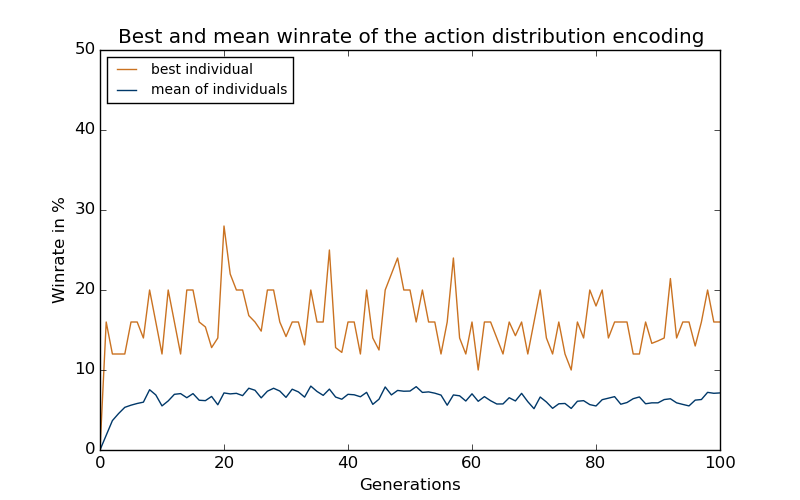
\includegraphics[scale=0.5]{../pictures/summary/actiondist-fitness.png}\\
                        \caption{Fitness Graph für die \\Wahrscheinlichkeitsverteilung}\label{fig:temp}
                    \end{figure}
                \end{multicols}
%                     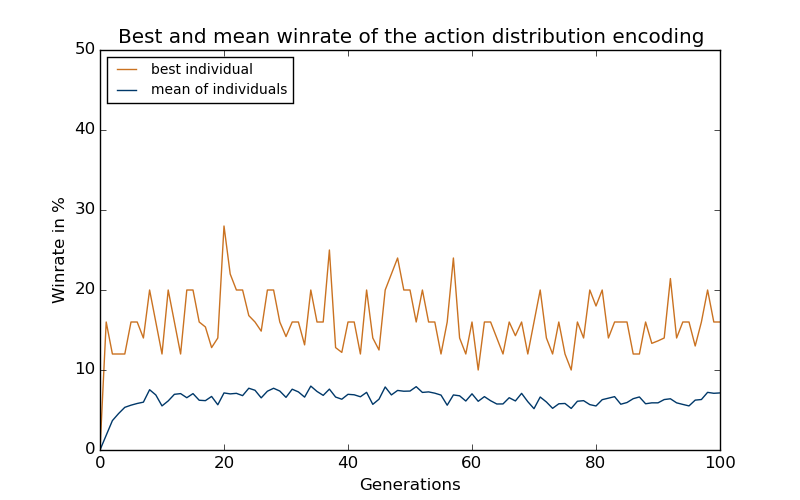
\includegraphics[scale=0.4]{../pictures/summary/actiondist-fitness.png}
%                     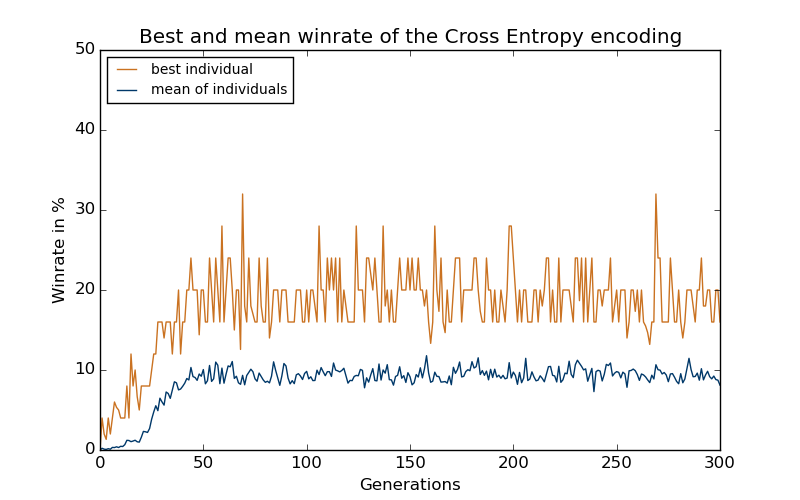
\includegraphics[scale=0.4]{../pictures/summary/cross-entropy-fitness.png}
%                     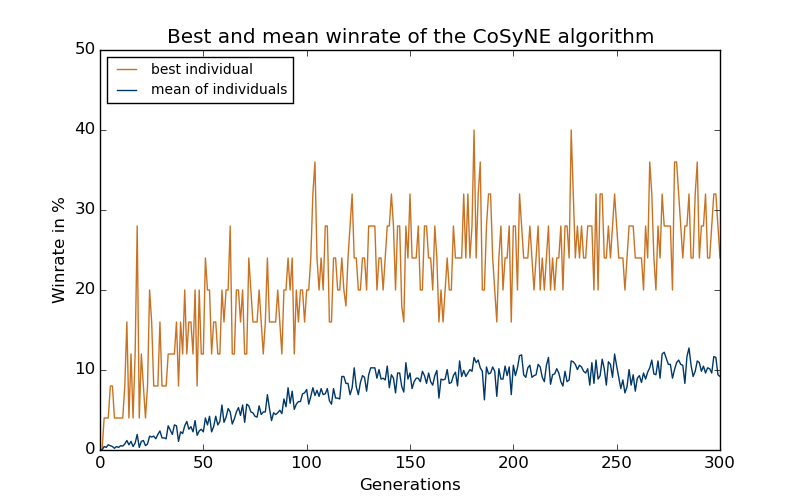
\includegraphics[scale=0.3]{../pictures/summary/cosyne-fitness.png}
%                     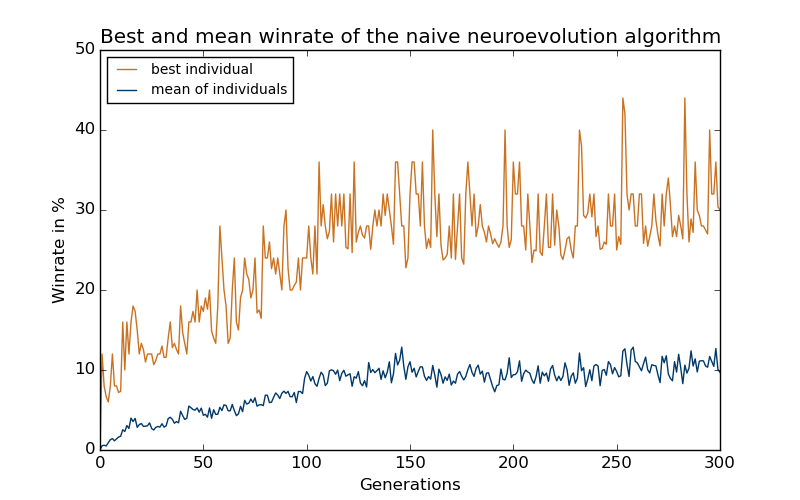
\includegraphics[scale=0.3]{../pictures/summary/neural-fitness.png}

            \subsubsection*{Cross Entropy}
                ``Graph zeigen, Interpretation bzw. Erklärung''
                ``Aggressivität''
                ``Nach ~ 50 Episoden stagniert''
            \subsubsection*{Neuroevolution}
                ``Graph zeigen, Interpretation bzw. Erklärung''
            \subsubsection*{CoSyNE}
                ``Graph zeigen, Interpretation bzw. Erklärung''
        \subsection{Vergleich}
            ``Sicherheit <-> Aggressivität steht im Kontra zur Stabilität der Algorithmen''\\
            ``Wenn Zeit ein Faktor wäre'' \\
            ``Wenn Sicherheit ein Faktor wäre'' \\


